\chapter{Introduction}
\label{sec:introduction}

\exercise
\begin{center}
	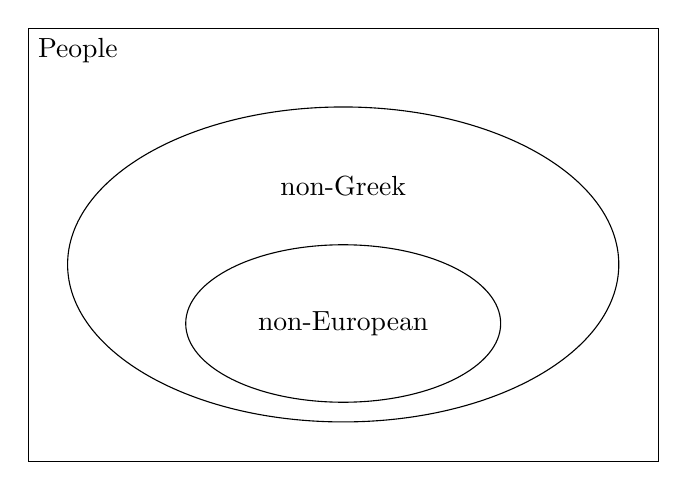
\begin{tikzpicture}
	\draw (0,0) rectangle (8,5.5);
	\draw (4,2.5) ellipse (3.5 and 2);
	\draw (4,1.75) ellipse (2 and 1);
	\draw (0,5.5) node[anchor = north west]{People};
	\draw (4,3.5) node[anchor = center]{non-Greek};
	\draw (4,1.75) node[anchor = center]{non-European};
	\end{tikzpicture}
\end{center}

\exercise
\begin{center}
	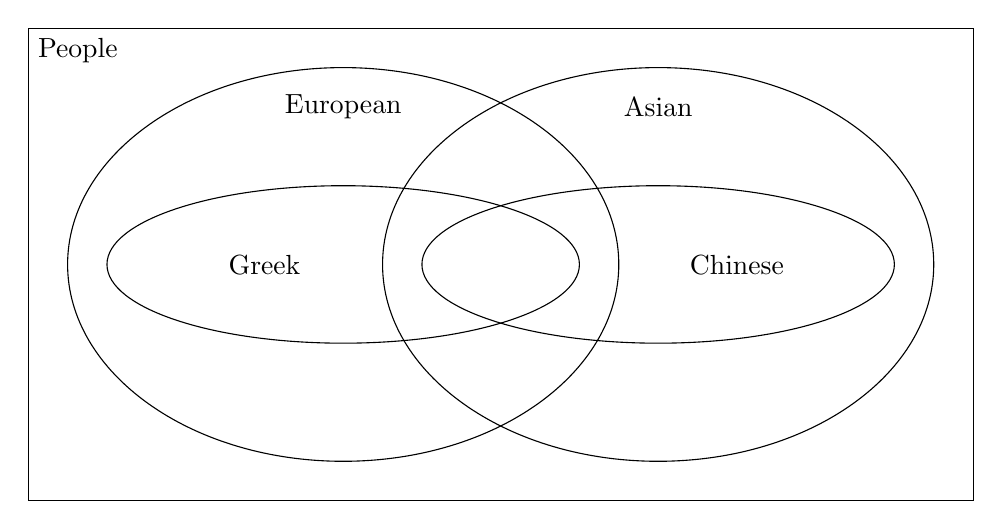
\begin{tikzpicture}
	\draw (0,0) rectangle (12,6);
	\draw (4,3) ellipse (3.5 and 2.5);
	\draw (8,3) ellipse (3.5 and 2.5);
	\draw (4,3) ellipse (3 and 1);
	\draw (8,3) ellipse (3 and 1);
	\draw (0,6) node[anchor = north west]{People};
	\draw (4,5) node[anchor = center]{European};
	\draw (8,5) node[anchor = center]{Asian};
	\draw (3,3) node[anchor = center]{Greek};
	\draw (9,3) node[anchor = center]{Chinese};
	\end{tikzpicture}
\end{center}

\exercise
statement $p$: $\sqrt{2} \in \R$ \\
statement $q$: $\sqrt{2}$ is not rational \\
statement $r$: $m$ and $n$ have no common divisor

\exercise
$f \circ (g \circ h)(w) = f \circ g(h(w)) = f(g(h(w))) = (f \circ g)(h(w))=(f \circ g) \circ h(w)$ \QED

\exercise
identity map definition: $\forall x \in \X, 1_X(x) = x$ \\
injective: $1_X(x_1) = 1_X(x_2) \Rightarrow x_1 = x_2$ \\
surjective: $\forall y \in \X, \exists x = y \in \X, 1_X(x) = y$ \\
injective $\wedge$ surjective $\Rightarrow$ bijective \QED

\problem
Assume, for the sake of contradiction, $\exists n \in \N$, such that $n$ is both odd and even. According to the definitions of even and odd numbers, we know that $\exists p \in \N, n = 2p+1$ and $\exists q \in \N, n = 2q$. Thus, $2p+1 = 2q$ and hence $q = p + 0.5$. Since $p \in \N$, $q = p + 0.5 \notin \N$, which leads to the contradiction with $q \in \N$. Therefore, $n$ cannot be both odd and even. \QED \\

\problem
\begin{enumerate}
\item $f$ has a left inverse if and only if it is injective:
\begin{itemize}
	\item Suppose $f$ has a left inverse $g_L$, \\
	$g_L:\Y \rightarrow \X$ such that $\forall x\in \X, g_L \circ f(x) = x$ \\
	$f(x_1)=f(x_2) \Rightarrow g_L(f(x_1)) = g_L(f(x_2)) \Rightarrow x_1 = x_2 \Rightarrow$ injective
	\item Suppose $f$ is injective, $\forall y \in \range{f}$, $\exists ! x \in \X, f(x) = y$. \\
	Construct $g_L(y) = \begin{cases}
	x & y \in \range{f} \\
	0 & otherwise
	\end{cases}$ \\
	Then $g_L(y)$ defines the left inverse function of $f$.
\end{itemize}

\item $f$ has a right inverse if and only if it is surjective:
\begin{itemize}
	\item Suppose $f$ has a right inverse $g_R$, $\forall y \in \Y, f \circ g_R(y) = y$. \\
	$\forall y \in \Y, \exists x = g(y) \in \X, \text{such that } f(x) = y \Rightarrow$ surjective
	\item Suppose $f$ is surjective, $\forall y \in \Y, \exists x \in \X, f(x) = y$. \\
	Let $g_R(y) = x$. If multiple $x$ exist, choose one of them. \\
	$f \circ g_R (y) = f(g_R(y)) = f(x) = y = 1_\Y(y)$ \\
	Therefore $g_R(y)$ defines the right inverse function of $f$.
\end{itemize}

\item $f$ is invertible if and only if it is bijective:
\begin{itemize}
	\item Suppose $f$ is invertible, there exist left and right inverse of $f$. Then $f$ is both injective and surjective, which implies $f$ is bijective.
	\item Suppose $f$ is bijective, we only need to prove $g = g_L = g_R$. \\
	$g_L(y) = g_L \circ 1_\Y(y) = g_L(1_\Y(y)) = g_L(f\circ g_R(y)) = (g_L \circ f) \circ g_R (y) = 1_\X \circ g_R (y) = g_R(y) \Rightarrow g_L = g_R$
\end{itemize}
\end{enumerate} \QED